\chapter{Puiden käsittely}

\index{puu@puu}

\key{Puu} on yhtenäinen, syklitön verkko,
jossa on $n$ solmua ja $n-1$ kaarta.
Jos puusta poistaa yhden kaaren, se ei ole enää yhtenäinen,
ja jos puuhun lisää yhden kaaren, se ei ole enää syklitön.
Puussa pätee myös aina, että
jokaisen kahden puun solmun välillä on yksikäsitteinen polku.

Esimerkiksi seuraavassa puussa on 7 solmua ja 6 kaarta:

\begin{center}
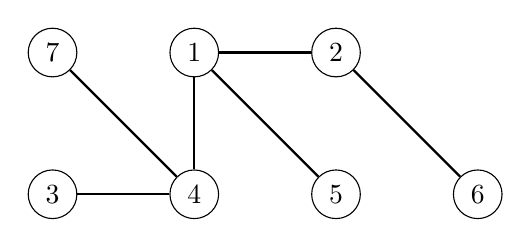
\begin{tikzpicture}[scale=0.9]
\node[draw, circle] (1) at (0,3) {$1$};
\node[draw, circle] (2) at (2,3) {$2$};
\node[draw, circle] (3) at (0,1) {$4$};
\node[draw, circle] (4) at (2,1) {$5$};
\node[draw, circle] (5) at (4,1) {$6$};
\node[draw, circle] (6) at (-2,3) {$7$};
\node[draw, circle] (7) at (-2,1) {$3$};
\path[draw,thick,-] (1) -- (2);
\path[draw,thick,-] (1) -- (3);
\path[draw,thick,-] (1) -- (4);
\path[draw,thick,-] (2) -- (5);
\path[draw,thick,-] (3) -- (6);
\path[draw,thick,-] (3) -- (7);
\end{tikzpicture}
\end{center}

\index{lehti@lehti}

Puun \key{lehdet} ovat solmut,
joiden aste on 1 eli joista lähtee vain yksi kaari.
Esimerkiksi yllä olevan puun lehdet ovat
solmut 3, 5, 6 ja 7.

\index{juuri@juuri}
\index{juurellinen puu@juurellinen puu}

Jos puu on \key{juurellinen}, yksi solmuista
on puun \key{juuri},
jonka alapuolelle muut solmut asettuvat.
Esimerkiksi jos yllä olevassa puussa valitaan
juureksi solmu 1, solmut asettuvat seuraavaan järjestykseen:

\begin{center}
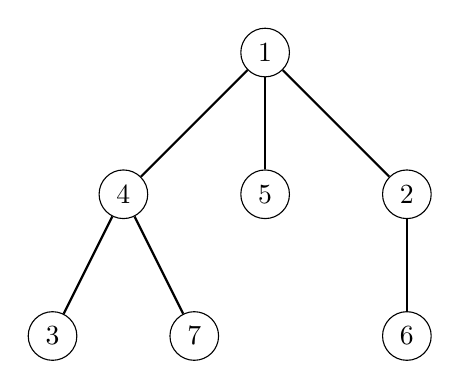
\begin{tikzpicture}[scale=0.9]
\node[draw, circle] (1) at (0,3) {$1$};
\node[draw, circle] (2) at (2,1) {$2$};
\node[draw, circle] (3) at (-2,1) {$4$};
\node[draw, circle] (4) at (0,1) {$5$};
\node[draw, circle] (5) at (2,-1) {$6$};
\node[draw, circle] (6) at (-3,-1) {$3$};
\node[draw, circle] (7) at (-1,-1) {$7$};
\path[draw,thick,-] (1) -- (2);
\path[draw,thick,-] (1) -- (3);
\path[draw,thick,-] (1) -- (4);
\path[draw,thick,-] (2) -- (5);
\path[draw,thick,-] (3) -- (6);
\path[draw,thick,-] (3) -- (7);
\end{tikzpicture}
\end{center}

\index{lapsi@lapsi}
\index{vanhempi@vanhempi}

Tällöin solmun \key{lapset}
ovat sen alemman tason naapurit
ja solmun \key{vanhempi}
on sen ylemmän tason naapuri.
Jokaisella solmulla on tasan yksi vanhempi,
paitsi juurella ei ole vanhempaa.
Esimerkiksi yllä olevassa puussa solmun 4
lapset ovat solmut 3 ja 7 ja solmun 4 vanhempi on solmu 1.

\index{alipuu@alipuu}

Juurellisen puun rakenne on rekursiivinen:
jokaisesta puun solmusta alkaa \key{alipuu},
jonka juurena on solmu itse ja johon kuuluvat
kaikki solmut, joihin solmusta pääsee kulkemalla alaspäin puussa.
Esimerkiksi solmun 4 alipuussa
ovat solmut 4, 3 ja 7.

\section{Puun läpikäynti}

Puun läpikäyntiin voi käyttää syvyyshakua ja
leveyshakua samaan
tapaan kuin yleisen verkon läpikäyntiin.
Erona on kuitenkin, että puussa ei ole silmukoita,
minkä ansiosta ei tarvitse huolehtia siitä,
että läpikäynti päätyisi tiettyyn
solmuun monesta eri suunnasta.

Tavallisin menetelmä puun läpikäyntiin on
valita tietty solmu juureksi ja aloittaa
siitä syvyyshaku.
Seuraava rekursiivinen funktio toteuttaa sen:

\begin{lstlisting}
void haku(int s, int e) {
    // solmun s käsittely tähän
    for (auto u : v[s]) {
        if (u != e) haku(u, s);
    }
}
\end{lstlisting}

Funktion parametrit ovat käsiteltävä solmu $s$
sekä edellinen käsitelty solmu $e$.
Parametrin $e$ ideana on varmistaa, että
läpikäynti etenee vain alaspäin puussa
sellaisiin solmuihin, joita ei ole vielä käsitelty.

Seuraava kutsu käy läpi puun aloittaen juuresta $x$:

\begin{lstlisting}
haku(x, 0);
\end{lstlisting}

Ensimmäisessä kutsussa $e=0$, koska läpikäynti
saa edetä juuresta kaikkiin suuntiin alaspäin.

\subsubsection{Dynaaminen ohjelmointi}

Puun läpikäyntiin voi myös yhdistää dynaamista
ohjelmointia ja laskea sen avulla jotakin tietoa puusta.
Dynaamisen ohjelmoinnin avulla voi esimerkiksi
laskea ajassa $O(n)$ jokaiselle solmulle,
montako solmua sen alipuussa
on tai kuinka pitkä on pisin solmusta
alaspäin jatkuva polku puussa.

Lasketaan esimerkiksi jokaiselle solmulle $s$
sen alipuun solmujen määrä $\texttt{c}[s]$.
Solmun alipuuhun kuuluvat solmu itse
sekä kaikki sen lasten alipuut.
Niinpä solmun alipuun solmujen määrä on
yhden suurempi kuin summa lasten
alipuiden solmujen määristä.
Laskennan voi toteuttaa seuraavasti:

\begin{lstlisting}
void haku(int s, int e) {
    c[s] = 1;
    for (auto u : v[s]) {
        if (u == e) continue;
        haku(u, s);
        c[s] += c[u];
    }
}
\end{lstlisting}

\section{Läpimitta}

\index{lzpimitta@läpimitta}

Puun \key{läpimitta} on pisin polku
kahden puussa olevan solmun välillä.
Esimerkiksi puussa
\begin{center}
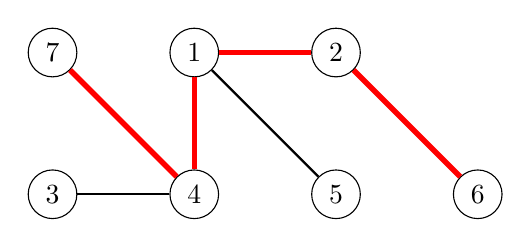
\begin{tikzpicture}[scale=0.9]
\node[draw, circle] (1) at (0,3) {$1$};
\node[draw, circle] (2) at (2,3) {$2$};
\node[draw, circle] (3) at (0,1) {$4$};
\node[draw, circle] (4) at (2,1) {$5$};
\node[draw, circle] (5) at (4,1) {$6$};
\node[draw, circle] (6) at (-2,3) {$7$};
\node[draw, circle] (7) at (-2,1) {$3$};
\path[draw,thick,-] (1) -- (2);
\path[draw,thick,-] (1) -- (3);
\path[draw,thick,-] (1) -- (4);
\path[draw,thick,-] (2) -- (5);
\path[draw,thick,-] (3) -- (6);
\path[draw,thick,-] (3) -- (7);

\path[draw,thick,-,color=red,line width=2pt] (6) -- (3);
\path[draw,thick,-,color=red,line width=2pt] (3) -- (1);
\path[draw,thick,-,color=red,line width=2pt] (1) -- (2);
\path[draw,thick,-,color=red,line width=2pt] (2) -- (5);
\end{tikzpicture}
\end{center}

läpimitta on 4, koska polku solmusta 3 solmuun 6
on pituudeltaan 4.
Läpimittaa vastaava polku ei ole
välttämättä yksikäsitteinen.
Esimerkiksi tässä puussa myös polku solmusta 7
solmuun 6 on pituudeltaan 4.

Käymme seuraavaksi läpi kaksi tehokasta
algoritmia puun läpimitan laskeminen.
Molemmat algoritmit laskevat läpimitan ajassa
$O(n)$.
Ensimmäinen algoritmi perustuu dynaamiseen
ohjelmointiin, ja toinen algoritmi
etsii kaukaisimmat solmut syvyyshakujen avulla.

\subsubsection{Algoritmi 1}

Algoritmin alussa
yksi solmuista valitaan puun juureksi.
Tämän jälkeen algoritmi laskee
jokaiseen solmuun,
kuinka pitkä on pisin polku,
joka alkaa jostakin lehdestä,
nousee kyseiseen solmuun asti
ja laskeutuu toiseen lehteen.
Pisin tällaisista poluista vastaa puun läpimittaa.

Esimerkissä pisin polku alkaa lehdestä 7,
nousee solmuun 1 asti ja laskeutuu
sitten alas lehteen 6:
\begin{center}
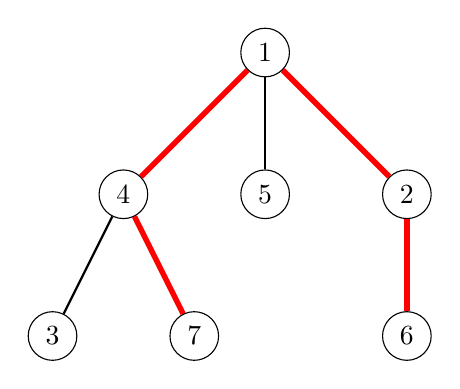
\begin{tikzpicture}[scale=0.9]
\node[draw, circle] (1) at (0,3) {$1$};
\node[draw, circle] (2) at (2,1) {$2$};
\node[draw, circle] (3) at (-2,1) {$4$};
\node[draw, circle] (4) at (0,1) {$5$};
\node[draw, circle] (5) at (2,-1) {$6$};
\node[draw, circle] (6) at (-3,-1) {$3$};
\node[draw, circle] (7) at (-1,-1) {$7$};
\path[draw,thick,-] (1) -- (2);
\path[draw,thick,-] (1) -- (3);
\path[draw,thick,-] (1) -- (4);
\path[draw,thick,-] (2) -- (5);
\path[draw,thick,-] (3) -- (6);
\path[draw,thick,-] (3) -- (7);

\path[draw,thick,-,color=red,line width=2pt] (7) -- (3);
\path[draw,thick,-,color=red,line width=2pt] (3) -- (1);
\path[draw,thick,-,color=red,line width=2pt] (1) -- (2);
\path[draw,thick,-,color=red,line width=2pt] (2) -- (5);
\end{tikzpicture}
\end{center}

Algoritmi laskee ensin dynaamisella ohjelmoinnilla
jokaiselle solmulle, kuinka pitkä on pisin solmu,
joka lähtee solmusta alaspäin.
Esimerkiksi yllä olevassa puussa pisin polku
solmusta 1 alaspäin on pituudeltaan 2
(vaihtoehdot $1 \rightarrow 4 \rightarrow 3$,
$1 \rightarrow 4 \rightarrow 7$ ja $1 \rightarrow 2 \rightarrow 6$).

Tämän jälkeen algoritmi laskee kullekin solmulle,
kuinka pitkä on pisin polku, jossa solmu on käännekohtana.
Pisin tällainen polku syntyy valitsemalla kaksi lasta,
joista lähtee alaspäin mahdollisimman pitkä polku.
Esimerkiksi yllä olevassa puussa solmun 1 lapsista valitaan solmut 2 ja 4.

\subsubsection{Algoritmi 2}

Toinen tehokas tapa laskea puun läpimitta 
perustuu kahteen syvyyshakuun.
Ensin valitaan mikä tahansa solmu $a$ puusta
ja etsitään siitä kaukaisin solmu $b$
syvyyshaulla.
Tämän jälkeen etsitään $b$:stä kaukaisin
solmu $c$ syvyyshaulla.
Puun läpimitta on etäisyys $b$:n ja $c$:n välillä.

Esimerkissä $a$, $b$ ja $c$ voisivat olla:
\begin{center}
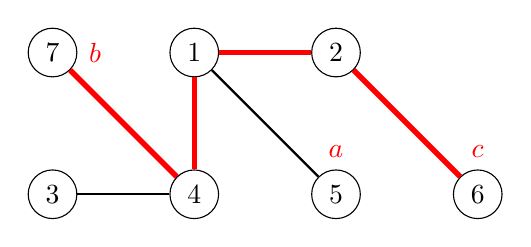
\begin{tikzpicture}[scale=0.9]
\node[draw, circle] (1) at (0,3) {$1$};
\node[draw, circle] (2) at (2,3) {$2$};
\node[draw, circle] (3) at (0,1) {$4$};
\node[draw, circle] (4) at (2,1) {$5$};
\node[draw, circle] (5) at (4,1) {$6$};
\node[draw, circle] (6) at (-2,3) {$7$};
\node[draw, circle] (7) at (-2,1) {$3$};
\path[draw,thick,-] (1) -- (2);
\path[draw,thick,-] (1) -- (3);
\path[draw,thick,-] (1) -- (4);
\path[draw,thick,-] (2) -- (5);
\path[draw,thick,-] (3) -- (6);
\path[draw,thick,-] (3) -- (7);
\node[color=red] at (2,1.6) {$a$};
\node[color=red] at (-1.4,3) {$b$};
\node[color=red] at (4,1.6) {$c$};

\path[draw,thick,-,color=red,line width=2pt] (6) -- (3);
\path[draw,thick,-,color=red,line width=2pt] (3) -- (1);
\path[draw,thick,-,color=red,line width=2pt] (1) -- (2);
\path[draw,thick,-,color=red,line width=2pt] (2) -- (5);
\end{tikzpicture}
\end{center}

Menetelmä on tyylikäs, mutta miksi se toimii?

Tässä auttaa tarkastella puuta niin,
että puun läpimittaa vastaava polku on
levitetty vaakatasoon ja muut puun osat
riippuvat siitä alaspäin:
\begin{center}
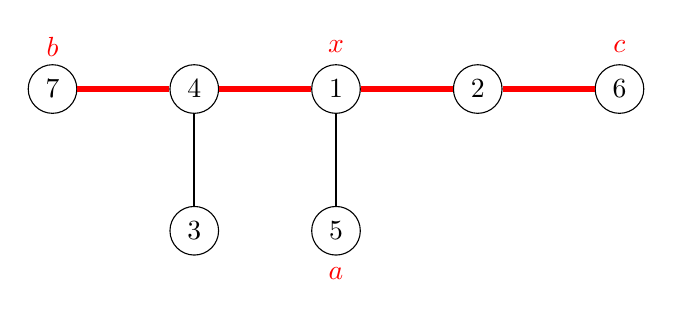
\begin{tikzpicture}[scale=0.9]
\node[draw, circle] (1) at (2,1) {$1$};
\node[draw, circle] (2) at (4,1) {$2$};
\node[draw, circle] (3) at (0,1) {$4$};
\node[draw, circle] (4) at (2,-1) {$5$};
\node[draw, circle] (5) at (6,1) {$6$};
\node[draw, circle] (6) at (0,-1) {$3$};
\node[draw, circle] (7) at (-2,1) {$7$};
\path[draw,thick,-] (1) -- (2);
\path[draw,thick,-] (1) -- (3);
\path[draw,thick,-] (1) -- (4);
\path[draw,thick,-] (2) -- (5);
\path[draw,thick,-] (3) -- (6);
\path[draw,thick,-] (3) -- (7);
\node[color=red] at (2,-1.6) {$a$};
\node[color=red] at (-2,1.6) {$b$};
\node[color=red] at (6,1.6) {$c$};
\node[color=red] at (2,1.6) {$x$};

\path[draw,thick,-,color=red,line width=2pt] (7) -- (3);
\path[draw,thick,-,color=red,line width=2pt] (3) -- (1);
\path[draw,thick,-,color=red,line width=2pt] (1) -- (2);
\path[draw,thick,-,color=red,line width=2pt] (2) -- (5);
\end{tikzpicture}
\end{center}

Solmu $x$ on kohta,
jossa polku solmusta $a$ liittyy
läpimittaa vastaavaan polkuun.
Kaukaisin solmu $a$:sta
on solmu $b$, solmu $c$
tai jokin muu solmu, joka
on ainakin yhtä kaukana solmusta $x$.
Niinpä tämä solmu on aina sopiva
valinta läpimittaa vastaavan polun
toiseksi päätesolmuksi.

\section{Solmujen etäisyydet}

Vaikeampi tehtävä on laskea
jokaiselle puun solmulle
jokaiseen suuntaan, mikä on suurin
etäisyys johonkin kyseisessä suunnassa
olevaan solmuun.
Osoittautuu, että tämäkin tehtävä ratkeaa
ajassa $O(n)$ dynaamisella ohjelmoinnilla.

\begin{samepage}
Esimerkkipuussa etäisyydet ovat:
\begin{center}
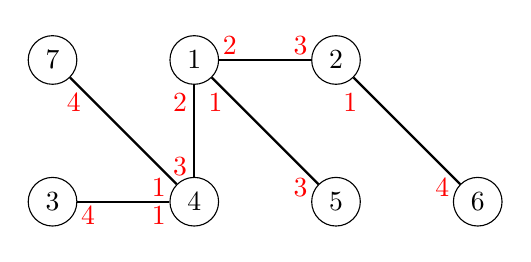
\begin{tikzpicture}[scale=0.9]
\node[draw, circle] (1) at (0,3) {$1$};
\node[draw, circle] (2) at (2,3) {$2$};
\node[draw, circle] (3) at (0,1) {$4$};
\node[draw, circle] (4) at (2,1) {$5$};
\node[draw, circle] (5) at (4,1) {$6$};
\node[draw, circle] (6) at (-2,3) {$7$};
\node[draw, circle] (7) at (-2,1) {$3$};
\path[draw,thick,-] (1) -- (2);
\path[draw,thick,-] (1) -- (3);
\path[draw,thick,-] (1) -- (4);
\path[draw,thick,-] (2) -- (5);
\path[draw,thick,-] (3) -- (6);
\path[draw,thick,-] (3) -- (7);
\node[color=red] at (0.5,3.2) {$2$};
\node[color=red] at (0.3,2.4) {$1$};
\node[color=red] at (-0.2,2.4) {$2$};
\node[color=red] at (-0.2,1.5) {$3$};
\node[color=red] at (-0.5,1.2) {$1$};
\node[color=red] at (-1.7,2.4) {$4$};
\node[color=red] at (-0.5,0.8) {$1$};
\node[color=red] at (-1.5,0.8) {$4$};
\node[color=red] at (1.5,3.2) {$3$};
\node[color=red] at (1.5,1.2) {$3$};
\node[color=red] at (3.5,1.2) {$4$};
\node[color=red] at (2.2,2.4) {$1$};
\end{tikzpicture}
\end{center}
\end{samepage}
Esimerkiksi solmussa 4
kaukaisin solmu ylöspäin mentäessä
on solmu 6, johon etäisyys on 3 käyttäen
polkua $4 \rightarrow 1 \rightarrow 2 \rightarrow 6$.

\begin{samepage}
Tässäkin tehtävässä hyvä lähtökohta on
valita jokin solmu puun juureksi,
jolloin kaikki etäisyydet alaspäin
saa laskettua dynaamisella ohjelmoinnilla:
\begin{center}
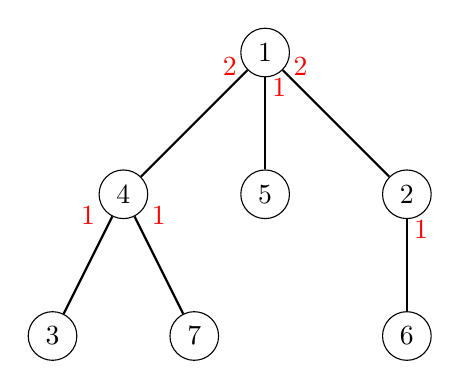
\begin{tikzpicture}[scale=0.9]
\node[draw, circle] (1) at (0,3) {$1$};
\node[draw, circle] (2) at (2,1) {$2$};
\node[draw, circle] (3) at (-2,1) {$4$};
\node[draw, circle] (4) at (0,1) {$5$};
\node[draw, circle] (5) at (2,-1) {$6$};
\node[draw, circle] (6) at (-3,-1) {$3$};
\node[draw, circle] (7) at (-1,-1) {$7$};
\path[draw,thick,-] (1) -- (2);
\path[draw,thick,-] (1) -- (3);
\path[draw,thick,-] (1) -- (4);
\path[draw,thick,-] (2) -- (5);
\path[draw,thick,-] (3) -- (6);
\path[draw,thick,-] (3) -- (7);

\node[color=red] at (-2.5,0.7) {$1$};
\node[color=red] at (-1.5,0.7) {$1$};

\node[color=red] at (2.2,0.5) {$1$};

\node[color=red] at (-0.5,2.8) {$2$};
\node[color=red] at (0.2,2.5) {$1$};
\node[color=red] at (0.5,2.8) {$2$};
\end{tikzpicture}
\end{center}
\end{samepage}

Jäljelle jäävä tehtävä on laskea etäisyydet ylöspäin.
Tämä onnistuu tekemällä puuhun toinen läpikäynti,
joka pitää mukana tietoa,
mikä on suurin etäisyys solmun vanhemmasta
johonkin toisessa suunnassa olevaan solmuun.

Esimerkiksi solmun 2
suurin etäisyys ylöspäin on yhtä suurempi
kuin solmun 1 suurin etäisyys
johonkin muuhun suuntaan kuin solmuun 2:
\begin{center}
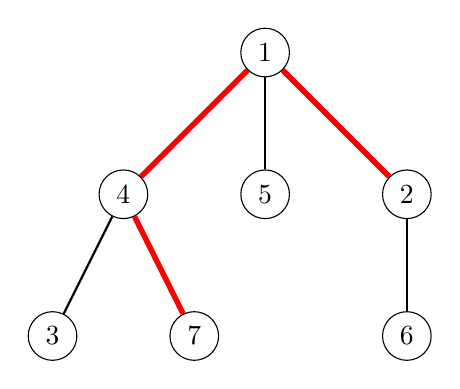
\begin{tikzpicture}[scale=0.9]
\node[draw, circle] (1) at (0,3) {$1$};
\node[draw, circle] (2) at (2,1) {$2$};
\node[draw, circle] (3) at (-2,1) {$4$};
\node[draw, circle] (4) at (0,1) {$5$};
\node[draw, circle] (5) at (2,-1) {$6$};
\node[draw, circle] (6) at (-3,-1) {$3$};
\node[draw, circle] (7) at (-1,-1) {$7$};
\path[draw,thick,-] (1) -- (2);
\path[draw,thick,-] (1) -- (3);
\path[draw,thick,-] (1) -- (4);
\path[draw,thick,-] (2) -- (5);
\path[draw,thick,-] (3) -- (6);
\path[draw,thick,-] (3) -- (7);

\path[draw,thick,-,color=red,line width=2pt] (1) -- (2);
\path[draw,thick,-,color=red,line width=2pt] (1) -- (3);
\path[draw,thick,-,color=red,line width=2pt] (3) -- (7);

\end{tikzpicture}
\end{center}
Lopputuloksena on etäisyydet kaikista solmuista
kaikkiin suuntiin:
\begin{center}
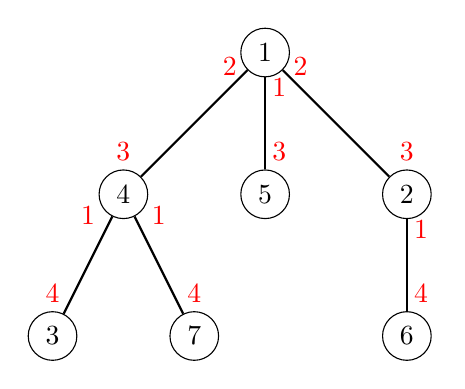
\begin{tikzpicture}[scale=0.9]
\node[draw, circle] (1) at (0,3) {$1$};
\node[draw, circle] (2) at (2,1) {$2$};
\node[draw, circle] (3) at (-2,1) {$4$};
\node[draw, circle] (4) at (0,1) {$5$};
\node[draw, circle] (5) at (2,-1) {$6$};
\node[draw, circle] (6) at (-3,-1) {$3$};
\node[draw, circle] (7) at (-1,-1) {$7$};
\path[draw,thick,-] (1) -- (2);
\path[draw,thick,-] (1) -- (3);
\path[draw,thick,-] (1) -- (4);
\path[draw,thick,-] (2) -- (5);
\path[draw,thick,-] (3) -- (6);
\path[draw,thick,-] (3) -- (7);

\node[color=red] at (-2.5,0.7) {$1$};
\node[color=red] at (-1.5,0.7) {$1$};

\node[color=red] at (2.2,0.5) {$1$};

\node[color=red] at (-0.5,2.8) {$2$};
\node[color=red] at (0.2,2.5) {$1$};
\node[color=red] at (0.5,2.8) {$2$};

\node[color=red] at (-3,-0.4) {$4$};
\node[color=red] at (-1,-0.4) {$4$};
\node[color=red] at (-2,1.6) {$3$};
\node[color=red] at (2,1.6) {$3$};

\node[color=red] at (2.2,-0.4) {$4$};
\node[color=red] at (0.2,1.6) {$3$};
\end{tikzpicture}
\end{center}
% 
% Kummankin läpikäynnin aikavaativuus on $O(n)$,
% joten algoritmin kokonais\-aikavaativuus on $O(n)$.

\section{Binääripuut}

\index{binxxripuu@binääripuu}

\begin{samepage}
\key{Binääripuu} on juurellinen puu,
jonka jokaisella solmulla on vasen ja oikea alipuu.
On mahdollista, että alipuu on tyhjä,
jolloin puu ei jatku siitä pidemmälle alaspäin.
Niinpä jokaisella solmulla on 0, 1 tai 2 lasta.

Esimerkiksi seuraava puu on binääripuu:

\begin{center}
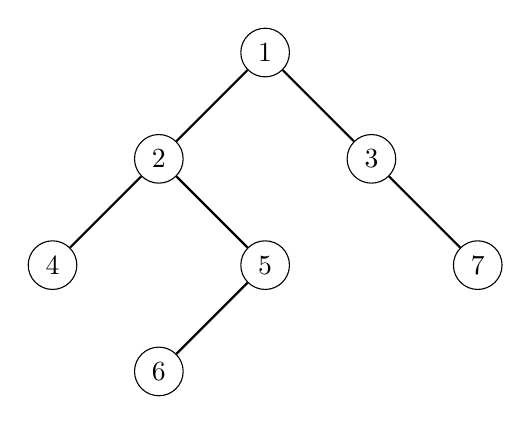
\begin{tikzpicture}[scale=0.9]
\node[draw, circle] (1) at (0,0) {$1$};
\node[draw, circle] (2) at (-1.5,-1.5) {$2$};
\node[draw, circle] (3) at (1.5,-1.5) {$3$};
\node[draw, circle] (4) at (-3,-3) {$4$};
\node[draw, circle] (5) at (0,-3) {$5$};
\node[draw, circle] (6) at (-1.5,-4.5) {$6$};
\node[draw, circle] (7) at (3,-3) {$7$};

\path[draw,thick,-] (1) -- (2);
\path[draw,thick,-] (1) -- (3);
\path[draw,thick,-] (2) -- (4);
\path[draw,thick,-] (2) -- (5);
\path[draw,thick,-] (5) -- (6);
\path[draw,thick,-] (3) -- (7);
\end{tikzpicture}
\end{center}
\end{samepage}

Binääripuun solmuilla on kolme luontevaa järjestystä,
jotka syntyvät rekursiivisesta läpikäynnistä:

\index{esijxrjestys@esijärjestys}
\index{sisxjxrjestys@sisäjärjestys}
\index{jxlkijxrjestys@jälkijärjestys}

\begin{itemize}
\item \key{esijärjestys}: juuri, vasen alipuu, oikea alipuu
\item \key{sisäjärjestys}: vasen alipuu, juuri, oikea alipuu
\item \key{jälkijärjestys}: vasen alipuu, oikea alipuu, juuri
\end{itemize}

Esimerkissä kuvatun puun esijärjestys on
$(1,2,4,5,6,3,7)$,
sisäjärjestys on $(4,2,6,5,1,3,7)$
ja jälkijärjestys on $(4,6,5,2,7,3,1)$.

Osoittautuu, että tietämällä puun esijärjestyksen
ja sisäjärjestyksen voi päätellä puun koko rakenteen.
Esimerkiksi yllä oleva puu on ainoa mahdollinen
puu, jossa esijärjestys on
$(1,2,4,5,6,3,7)$ ja sisäjärjestys on $(4,2,6,5,1,3,7)$.
Vastaavasti myös jälkijärjestys ja sisäjärjestys
määrittävät puun rakenteen.

Tilanne on toinen, jos tiedossa on vain
esijärjestys ja jälkijärjestys.
Nämä järjestykset eivät
kuvaa välttämättä puuta yksikäsitteisesti.
Esimerkiksi molemmissa puissa

\begin{center}
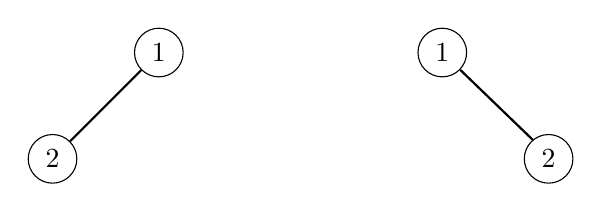
\begin{tikzpicture}[scale=0.9]
\node[draw, circle] (1) at (0,0) {$1$};
\node[draw, circle] (2) at (-1.5,-1.5) {$2$};
\path[draw,thick,-] (1) -- (2);

\node[draw, circle] (1b) at (0+4,0) {$1$};
\node[draw, circle] (2b) at (1.5+4,-1.5) {$2$};
\path[draw,thick,-] (1b) -- (2b);
\end{tikzpicture}
\end{center}

esijärjestys on $(1,2)$ ja jälkijärjestys on $(2,1)$,
mutta siitä huolimatta puiden rakenteet eivät ole samat.

